% Титульный лист (ГОСТ Р 7.0.11-2001, 5.1)
\thispagestyle{empty}%
\begin{center}%
\MakeUppercase{Московский государственный университет}\\
имени \MakeUppercase{М.В. Ломоносова}\\
\end{center}%
%
\vspace{0pt plus4fill} %число перед fill = кратность относительно некоторого расстояния fill, кусками которого заполнены пустые места
\begin{flushright}%

\textit {На правах рукописи}

% \textsl {УДК \thesisUdk}
\end{flushright}%
%
\vspace{0pt plus6fill} %число перед fill = кратность относительно некоторого расстояния fill, кусками которого заполнены пустые места
\begin{center}%
{\large Герасимов Кирилл Вячеславович}
\end{center}%
%
\vspace{0pt plus1fill} %число перед fill = кратность относительно некоторого расстояния fill, кусками которого заполнены пустые места
\begin{center}%
\textbf{ДИНАМИКА РОЛИКОНЕСУЩЕГО ЭКИПАЖА \\ С УЧЕТОМ ИНЕРЦИИ РОЛИКОВ И ТРЕНИЯ}

 \vspace{0pt plus6fill} %число перед fill = кратность относительно некоторого расстояния fill, кусками которого заполнены пустые места
% {%\small
% Специальность 
01.02.01~---~теоретическая механика
% }

\vspace{0pt plus4fill} %число перед fill = кратность относительно некоторого расстояния fill, кусками которого заполнены пустые места
АВТОРЕФЕРАТ \\ диссертации на соискание ученой степени \\ кандидата физико-математических наук

\end{center}%
%
\vspace{0pt plus4fill} %число перед fill = кратность относительно некоторого расстояния fill, кусками которого заполнены пустые места
%\begin{flushright}%
%Научные руководители:

%д.ф.-м.н. проф. Косенко И.И.\\
%к.ф.-м.н. доц. Зобова А.А.

%\end{flushright}%
%
\vspace{0pt plus4fill} %число перед fill = кратность относительно некоторого расстояния fill, кусками которого заполнены пустые места
\begin{center}%
{Москва~--- 2018}
\end{center}%
\newpage

% оборотная сторона обложки
\thispagestyle{empty}
\newgeometry{top=1.5cm,bottom=1cm,left=2cm}
\begin{center}
    Работа~выполнена~на~кафедре теоретической~механики~и мехатроники механико-математического~факультета~МГУ~имени~М.В.Ломоносова
\end{center}

\par\bigskip
%\begin{table}[h] % считается не очень правильным использовать окружение table, не задавая caption
    \noindent%
    \begin{tabular}{@{}p{5cm}p{16cm}}
        \textbf{Научные}               & --- Косенко Иван Иванович, \\
        \textbf{руководители:}         & доктор физико-математических наук,\\
                                       & --- Зобова Александра Александровна,\\
                                       & кандидат физико-математических наук
        \vspace{4mm} \\
        \textbf{Официальные}            & --- Кобрин Александр Исаакович, \\
        \textbf{оппоненты:}             & доктор физико-математических наук, профессор, \\
                                        & Институт энергомашиностроения и механики, \\
                                        & кафедра робототехники, мехатроники, динамики \\
                                        \vspace{4mm}
                                        & и прочности машин НИУ МЭИ, профессор \\
                                        & --- Холостова Ольга Владимировна, \\
                                        & доктор физико-математических наук, профессор, \\
                                        & кафедра ``Мехатроника и теоретическая механика'' \\
                                        \vspace{4mm}
                                        & НИУ МАИ, профессор \\
                                        & --- Никонов Василий Иванович, \\
                                        & кандидат физико-математических наук, \\
                                        & Вычислительный центр им. А.А. Дородницына РАН, \\
                                        & младший научный сотрудник\\
                                        \vspace{4mm}
    \end{tabular}  
%\end{table}
\par\bigskip

\vspace{-25pt}
Защита диссертации состоится <<14>> декабря 2018 г. в 17 часов на~заседании диссертационного совета МГУ.01.10 Московского государственного университета им. М.В.Ломоносова по~адресу: 119991, Москва, Ленинские горы, д. 1, Главное здание МГУ, механико-математический факультет, аудитория 16-10.

E-mail: msu.01.1@mech.math.msu.su

С диссертацией можно ознакомиться в отделе диссертаций научной библиотеки МГУ имени М.В.Ломоносова (Ломоносовский просп., д. 27) и на сайте ИАС <<ИСТИНА>>: https://istina.msu.ru/dissertations/154204063/

Автореферат разослан <<\underline{\hspace{1.2cm}}>>\underline{\hspace{4cm}} 20\underline{\hspace{1cm}}г.


%\begin{table} [h] % считается не очень правильным использовать окружение table, не задавая caption
\par\bigskip
    \noindent%
    \begin{tabular}{p{12cm}cr}
        \begin{tabular}{p{12cm}}
            Ученый секретарь  \\
            диссертационного совета МГУ.01.10 \\
            кандидат физико-математических наук
        \end{tabular} 
    &
        \hspace{-60pt}
        \begin{tabular}{c}
            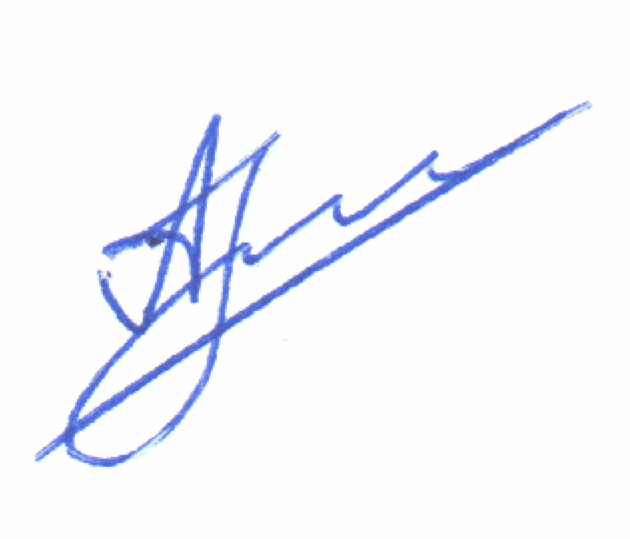
\includegraphics[height=2cm]{content/pic/new/sign.png}
        \end{tabular} 
    &
        \begin{tabular}{r}
            \\
            \\
            А.А. Зобова
        \end{tabular} 
    \end{tabular}
%\end{table}
    \restoregeometry
\newpage